\documentclass[12pt, a4paper]{article}
\usepackage[utf8]{inputenc}
\usepackage[english]{babel}
\usepackage{amsmath}
\usepackage{amsfonts}
\usepackage{amssymb}
\usepackage{csquotes}
\usepackage{mathtools}
\usepackage{graphicx}
\usepackage{geometry}
\usepackage{setspace}
\usepackage{longtable}
\usepackage{float}
\usepackage{comment}
\usepackage{listings}
\usepackage{fancyhdr}
\usepackage{blindtext}
\usepackage[colorlinks=true, allcolors=blue]{hyperref}

\usepackage[style=authoryear]{biblatex}
\addbibresource{Bibliography.bib}

\geometry{top = 2.5cm, bottom = 2.5cm, left= 3cm, right= 3cm}

\fancypagestyle{mystyle}
{
    \rhead{Experiment 4}
    \lfoot{Lee Farrugia}
    \cfoot{}
    \rfoot{Page \thepage}
    \renewcommand{\headrulewidth}{0pt}
    \renewcommand{\footrulewidth}{0.5pt}
}

\fancypagestyle{titlepagestyle}
{
    \fancyhf{}
    \lfoot{Lee Farrugia}
    \cfoot{}
    \rfoot{Page \thepage}
    \renewcommand{\headrulewidth}{0pt}
    \renewcommand{\footrulewidth}{0.5pt}
}

\title{Adiabatic Constant of Air}
\author{Lee Farrugia \\ Experiment 4 \\ Group 1A}

\date{11$^{\text{th}}$ March 2022}

\begin{document}

\maketitle
\thispagestyle{titlepagestyle}
\pagestyle{mystyle}

\section*{Aim}
The aim of this experiment was to determine the the ratio of specific heat capacities of air using Clement and Desormes' method.

\section*{Diagram}
\begin{figure}[H]
    \centering
    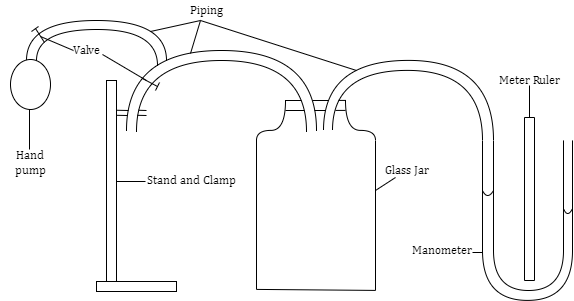
\includegraphics[width=\textwidth]{Experiment 4.png}
    \caption{Apparatus Set Up}
    \label{fig:set up}
\end{figure}

\section*{List of Apparatus}
Large glass jar, U-shaped manometer mounted with meter ruler, piping, two valves of different types, hand pump.

\section*{Language and Packages}
Python 3.9.7, Numpy, Pandas, Matplotlib.pyplot

\section*{Procedure}
\begin{enumerate}
    \item The valve connected to the hand pump was opened and air was pumped into the jar until the mark of 1 cm was reached. The difference between the two points was recorded as $h_0$.
    \item 15 minutes were left to pass so that the temperature inside the jar would be the same as the temperature outside the jar. The difference in height between the two sides of the manometer was recorded as $h_1$.
    \item The valve was opened and closed as soon as the levels in the manometer were about to equalise. 
    \item 2 minute were left to pass and the difference between the two values was recorded as $h_2$.
    \item This was repeated for a total of 5 readings, changing $h_0$ each time.
\end{enumerate}

\section*{Precautions}
\begin{itemize}
    \item[-] The readings from the meter ruler were taken at eye level.
    \item[-] Reading of the manometer were read from the meniscus of the level.
    \item[-] Apparatus was not kept in direct sunlight.
    \item[-] Doors and windows were closed as much as possible.
    \item[-] Multiple valves were used.
    \item[-] Any other opening to the jar was made sure to be closed as much as possible.
    \item[-] As much time as possible was elapsed for the air in the jar to reach thermal equilibrium. 
\end{itemize}

\section*{Sources of Error}
\begin{itemize}
    \item[-] Draft created by an open window and students walking about the lab, may have affected the thermal equilibrium.
    \item[-] The piping used was quite brittle thus may have leaked.
    \item[-] Previous uses of the apparatus with Potassium permanganate made it harder to read certain readings due to staining.
    \item[-] Due to repeated use, the valves may have not closed fully.
    \item[-] Not enough time may have no passed for the air in the jar to have reached thermal equilibrium. 
\end{itemize}

\section*{Data and Graphs}
\begin{longtable}{|c|c|c|c|}
\hline $h_0$/m & $h_1$/m & $h_2$/m & $d$/m\\
\hline \textpm 0.01 & \textpm 0.01 & \textpm 0.01 & \textpm 0.01\\ \hline
\endfirsthead

\hline $h_0$/m & $h_1$/m & $h_2$/m & $d$/m\\
\hline \textpm 0.01 & \textpm 0.01 & \textpm 0.01 & \textpm 0.01\\ \hline
\endhead

0.146 & 0.166 & 0.067 & 0.099\\ \hline
0.125 & 0.130 & 0.031 & 0.099\\ \hline
0.106 & 0.126 & 0.050 & 0.076\\ \hline
0.086 & 0.097 & 0.034 & 0.063\\ \hline
0.065 & 0.062 & 0.027 & 0.035\\ \hline
0.045 & 0.048 & 0.022 & 0.026\\ \hline

\caption{Data of $h_0$, $h_1$, $h_2$ and $(h_1-h_2)$}
\label{tab:Table 1}\\
\end{longtable}

\begin{figure}
    \centering
    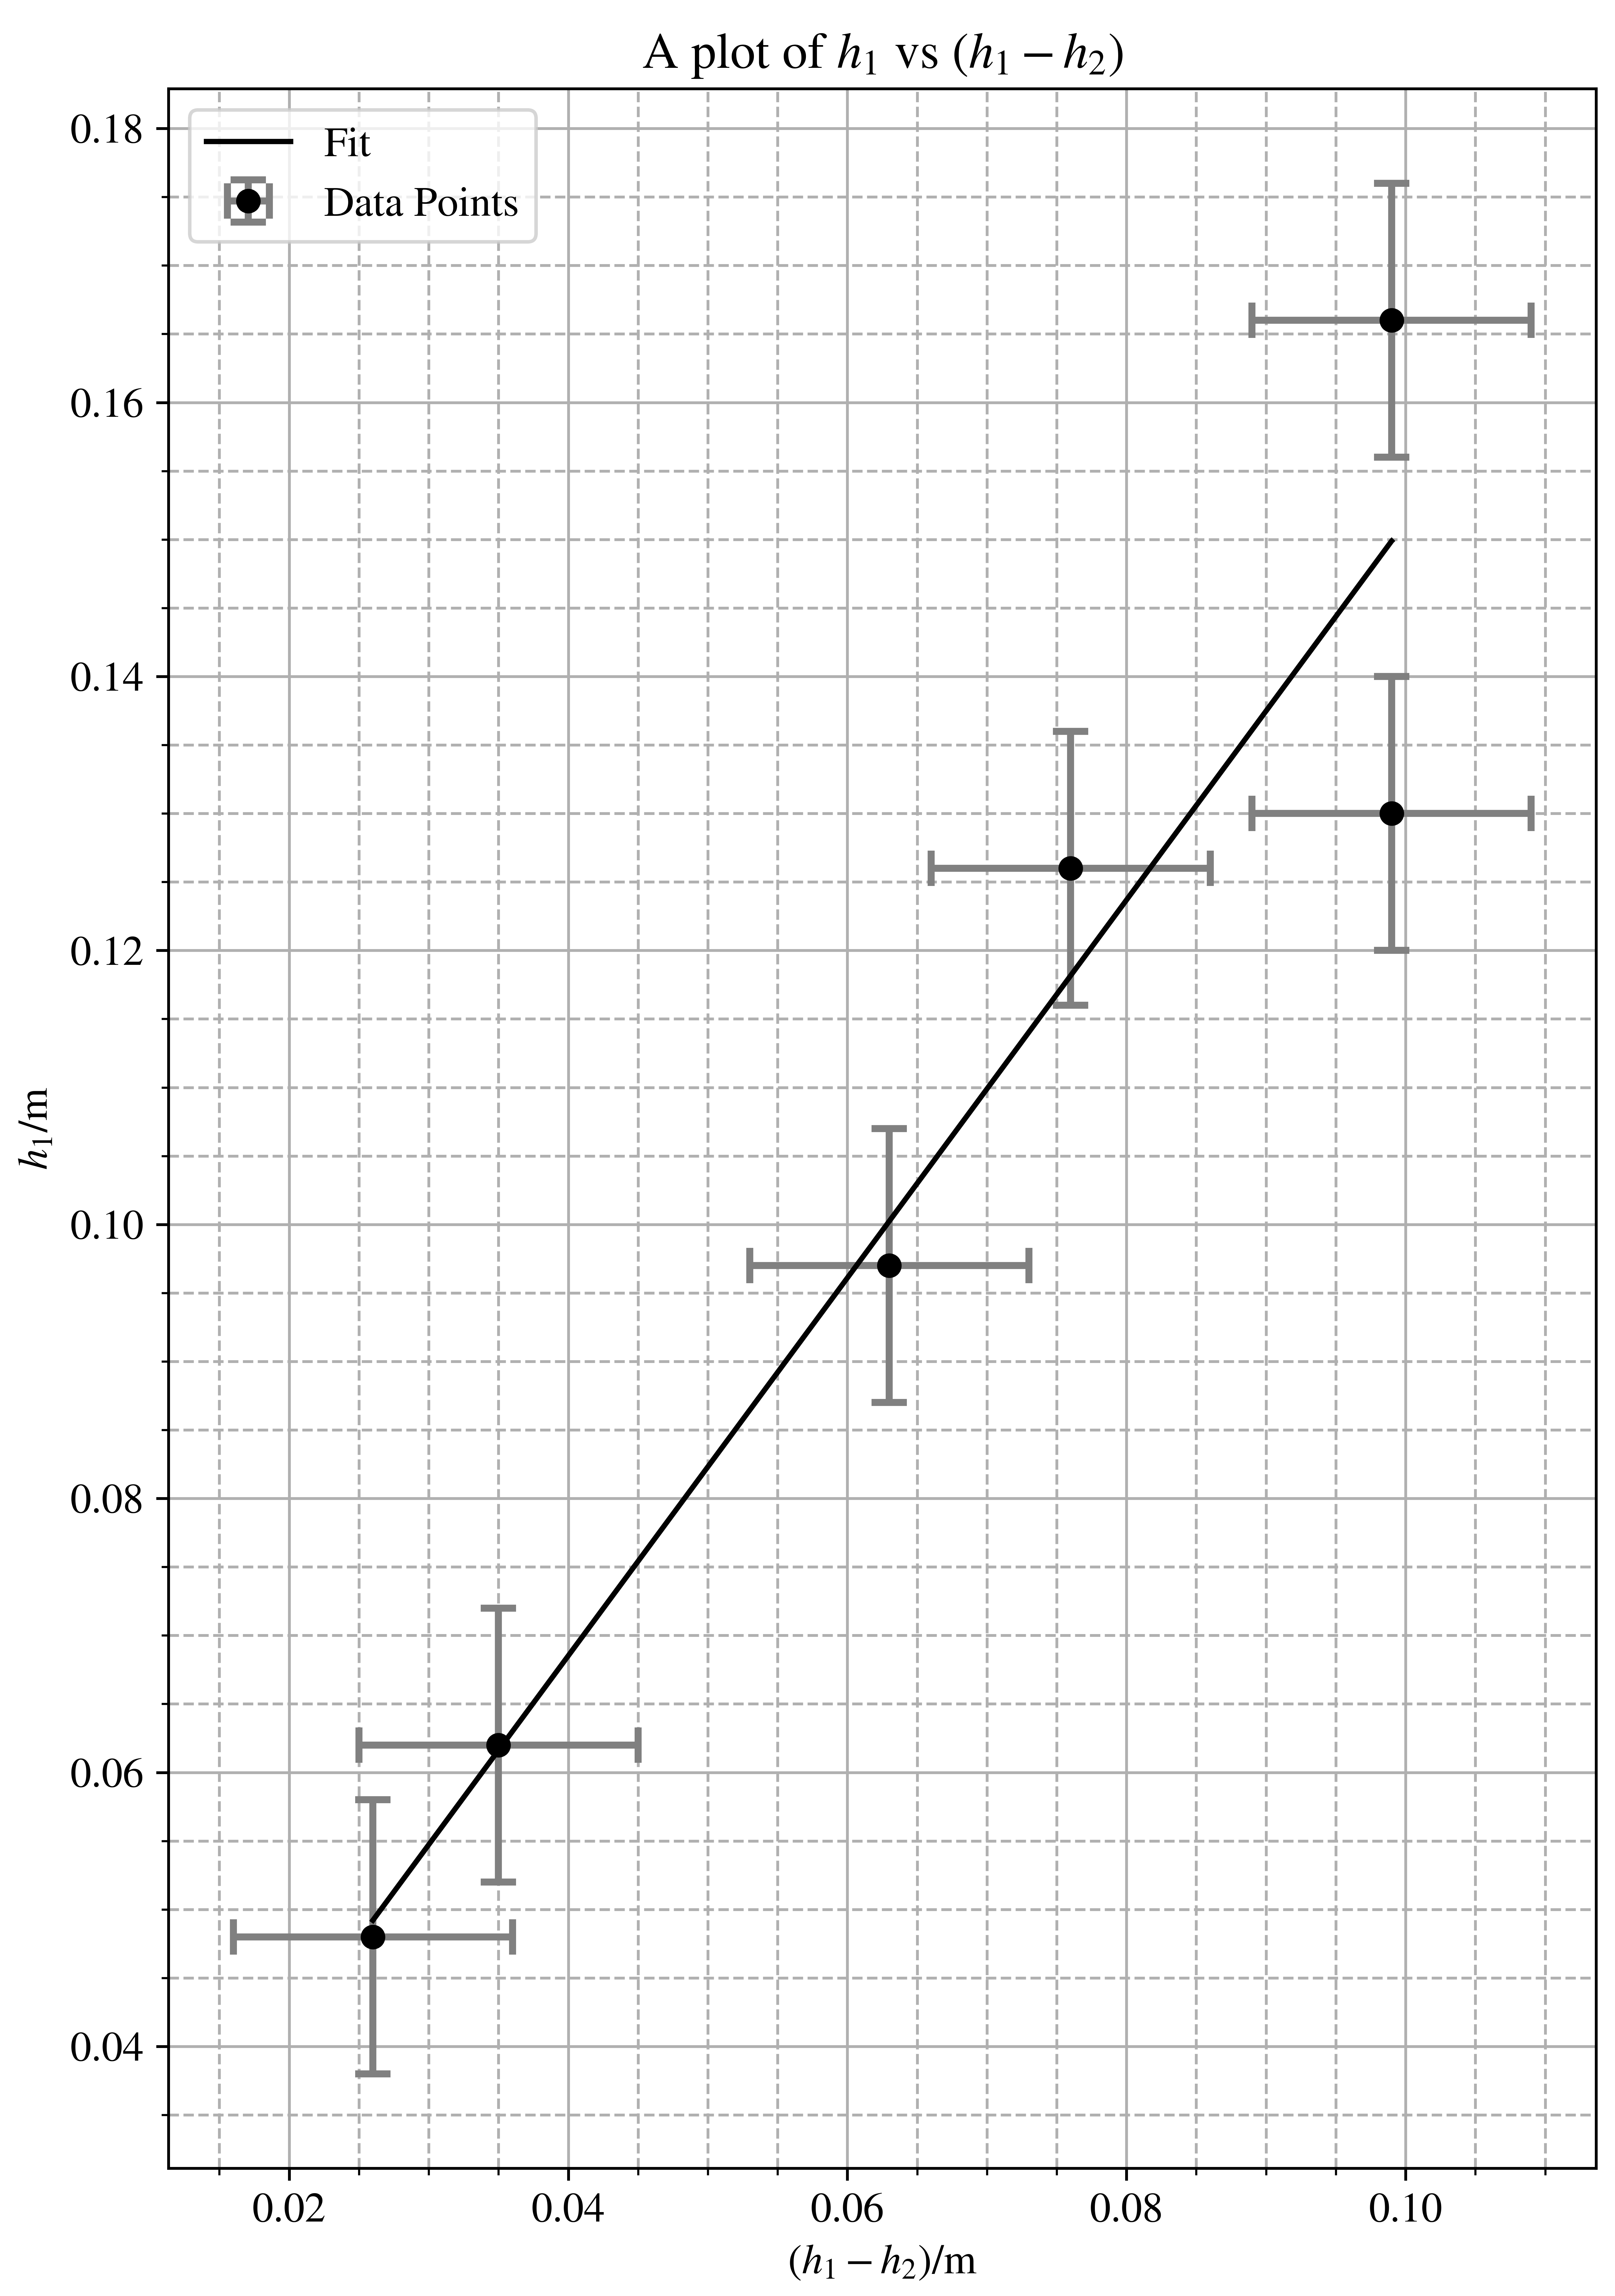
\includegraphics[width=\textwidth]{h1vsd.png}
    \caption{Graph of $h_1$/m vs $(h_1-h_2)$/m}
    \label{fig:Graph 1}
\end{figure}

\section*{Calculations}
The data gathered during the experiment were inputted into the program by using the following line of code:
\begin{lstlisting}
    data = pd.read_excel(`Experiment 4.xlsx').
\end{lstlisting}
$h_1$ and $h_2$ were defined using the following lines of code:
\begin{lstlisting}
    h1 = np.asarray(data[`h1']/100)
    h2 = np.asarray(data[`h2']/100)
    d = np.asarray(data[`d']/100),
\end{lstlisting}
where $d$ is the difference between $h_2$ and $h_1$.The equation given that links the ratio of the specific heat capacities of air was:
\begin{equation*}
    h_2 = \left(1-\frac{1}{\gamma}\right)h_1\,,
\end{equation*}
which when compared to the straight line equation of $y=\text{m}x+\text{c}$, we get that $y$ and $x$ correspond to $h_2$ and $h_1$ respectively. However, this was further adjusted in order to obtain the following equation:
\begin{equation*}
    h_1 = \frac{h1}{d}\gamma
\end{equation*}
Thus in order to obtain the line of best fit the following line of code were used:
\begin{lstlisting}
    coeffs, cov = np.polyfit(d, h2, deg=1, cov=True)
    poly_function = np.poly1d(coeffs)
    trendline = poly_function(d),
\end{lstlisting}
and the gradient was found by calling the correct position of the coeffs array by the following line of code:
\begin{lstlisting}
    m = coeffs[0].
\end{lstlisting}
The error of the gradient was found by square rooting the correct position in the co-variance matrix with the following line of code:
\begin{lstlisting}
    dm = np.sqrt(cov[0][0]).
\end{lstlisting}
From this it was found that $\gamma$ was found to be 1.37 with and error of 0.19. The error bars of $h_1$ and $h_2$ were found by using the following lines of code:
\begin{lstlisting}
    dh1 = 0.01
    dd = 0.01
    plt.errorbar(d, h1, xerr=dd, yerr=dh1, fmt=`o', 
                 color=`k', elinewidth=2, capthick=2, 
                 capsize=5, ecolor=`grey', 
                 label=`Data Points').
\end{lstlisting}
$dh1$ is the error of the $h_1$ and $dd$ is the error of $d$, and the these were taken to be the minimum readability from the meter ruler. The precision and accuracy of the values obtained were found using the following equations:
\begin{align*}
    \text{Precision}&=\frac{\text{Combined Error}}{\text{Experimental Value}} \times 100\% \\
    \smallskip
    \text{Accuracy} &= \frac{\text{Experimental Value}}{\text{Actual Value}} \times 100\% \,,
\end{align*}
which was done through the following lines of code:
\begin{lstlisting}
    precision = (dm/m) * 100
    accuracy = (m/1.4) * 100,
\end{lstlisting}
where $dm$ is the combined error of the experiment, $m$ is the value obtained for $\gamma$ and the 1.4 is the actual adiabatic constant of air. This resulted in a $14.06\%$ precision and $98.51\%$ accuracy.

\section*{Discussion}
The adiabatic constant of air $\gamma$ was found to be 1.37\textpm0.19, where actual value is 1.4 \parencite{muncaster}. The value obtained had an accuracy value of $98.51\%$, which implies that the value obtained is very accurate which can further seen from the fact that the value obtained was 1.37\textpm 0.19 while the actual value is 1.4. However, the precision value obtained from the experiment was $14.06\%$, which is larger than $10\%$, thus the values obtained were not as precise as one would have preferred. This can be further seen from the two outlying points on \ref{fig:Graph 1}. These two points on the line of best fit could be due to the fact that the temperature on the outside of the jar used, was varying somewhat due to the student and demonstrators walking about the laboratory, and that some of the windows and doors may have been left open. Although 15 minutes were left to pass between the initial reading and the second reading, this may have not been enough to allow the temperature inside the jar to reach thermal equilibrium with the temperature outside of the jar.

\medskip
\noindent
An adiabatic process can be defined as a process where no heat transfer occurs, i.e. no heat enter or leaves the system. This mean that the change heat energy called dQ, $\text{dQ}=0$. Thus this results that the only changes that happen is due to the change in pressure as there is a relation only in between pressure, $P$, and volume, $V$,\parencite{mashkevich}. A polytropic process is a process that occurs with heat transfer, however the heat transfer that occurs is reversible. Thus giving rise to the equation $\text{PVn}=\text{constant}$, where $P$ is the pressure, $V$ is the volume and n is the polytropic index number \parencite{muncaster}. As the system used follows an adiabatic process, one can not that in figure \ref{fig:Graph 1} the line generated does not pass through the points, thus meaning that not all data collected was as accurate as can be. Thus one can argue that a polytropic process would result in a more accurate result as the heat transfer into the system is reversible and thus would not affect the final outcome of the result \parencite{gresh}.

\section*{References:}
\printbibliography[heading=none]

\section*{Appendix}
\lstset{language=Python,
    showstringspaces=false,
    showtabs=false}
\begin{lstlisting}
import numpy as np
import pandas as pd
import matplotlib.pyplot as plt

# importing data
data = pd.read_excel(`Experiment 4.xlsx')
# defining relevant data
h1 = np.asarray(data[`h1']/100)
h2 = np.asarray(data[`h2']/100)
d = np.asarray(data[`d']/100)

# determining the eqaution of line of best fit
coeffs, cov = np.polyfit(d, h1, deg=1, cov=True)
poly_function = np.poly1d(coeffs)
trendline = poly_function(d)

# defining the gradient and error of gradient
m = coeffs[0]
dm = np.sqrt(cov[0][0])
# displaying values of gradient and error
print(f`Gamma is {m:.2f} with an error of {dm:.2f}')

# defining the minimum readability of the meter ruler
dh1 = 0.01
dd = 0.01

# finding the precision and accuracy 
  of the values of the value obtained
precision = (dm/m) * 100
accuracy = (m/1.4) * 100
print(f`With a precision of {precision:.2f}% 
        and an accuracy of {accuracy:.2f}%')

# defining the fonts and sizes to be used
plt.rcParams[`font.family'] = `STIXGeneral'
plt.rcParams[`mathtext.fontset'] = `stix'
plt.rcParams[`font.size'] = 12
plt.rcParams[`font.weight'] = `normal'

# defining the size of the figure
f = plt.figure(figsize=(7.3, 10.7))

# plotting errorbars and line of best fit
plt.errorbar(d, h1, xerr=dd, yerr=dh1, fmt=`o', color=`k',
             elinewidth=2, capthick=2, capsize=5,
             ecolor=`grey', label=`Data Points')
plt.plot(d, trendline, color=`k', label=`Fit')
# defining axis labels, title, grid, legend and showing plot
plt.minorticks_on()
plt.grid(b=True, which=`major', linestyle=`-')
plt.grid(b=True, which=`minor', linestyle=`--')
plt.xlabel(r`$(h_1-h_2)$/m')
plt.ylabel(r`$h_1$/m')
plt.title(r`A plot of $h_1$ vs $(h_1-h_2)$')
plt.legend()
plt.savefig(`h1vsd.png', dpi=800)
plt.show()


\end{lstlisting}

\end{document}
